%File: anonymous-submission-latex-2025.tex
\documentclass[letterpaper]{article} % DO NOT CHANGE THIS

\usepackage[submission]{aaai25}  % DO NOT CHANGE THIS
\usepackage{times}  % DO NOT CHANGE THIS
\usepackage{helvet}  % DO NOT CHANGE THIS
\usepackage{courier}  % DO NOT CHANGE THIS
\usepackage[hyphens]{url}  % DO NOT CHANGE THIS
\usepackage{graphicx} % DO NOT CHANGE THIS
\urlstyle{rm} % DO NOT CHANGE THIS
\def\UrlFont{\rm}  % DO NOT CHANGE THIS
\usepackage{natbib}  % DO NOT CHANGE THIS AND DO NOT ADD ANY OPTIONS TO IT
\usepackage{caption} % DO NOT CHANGE THIS AND DO NOT ADD ANY OPTIONS TO IT
\frenchspacing  % DO NOT CHANGE THIS
\setlength{\pdfpagewidth}{8.5in} % DO NOT CHANGE THIS
\setlength{\pdfpageheight}{11in} % DO NOT CHANGE THIS
%
% These are recommended to typeset algorithms but not required. See the subsubsection on algorithms. Remove them if you don't have algorithms in your paper.
\usepackage{algorithm}
\usepackage{algorithmic}
\usepackage{amsmath}
\usepackage{amsfonts}
\usepackage{amsthm}
\usepackage{mathrsfs}
\usepackage{mathtools}
\usepackage{booktabs}
\usepackage{lipsum}
\usepackage{listings}
\usepackage[acronym]{glossaries}
\usepackage{xspace}
\usepackage{circledsteps}
\usepackage{tikz}
\usetikzlibrary{arrows.meta, calc, positioning}
\tikzset{>=latex} % for LaTeX arrow head
\usepackage{pgfplots} % for the axis environment
\usepgfplotslibrary{fillbetween} % to fill an area under function
% define gaussian pdf and cdf
\pgfmathdeclarefunction{gauss}{3}{%
    \pgfmathparse{1/(#3*sqrt(2*pi))*exp(-((#1-#2)^2)/(2*#3^2))}%
}
\usepackage[outline]{contour} % halo around text
\usetikzlibrary{patterns}
\pgfplotsset{compat=1.12} % TikZ coordinates <-> axes coordinates
% https://tex.stackexchange.com/questions/240642/add-vertical-line-of-equation-x-2-and-shade-a-region-in-graph-by-pgfplots

\usepackage{environ}
\usepackage{import}
\usepackage{pgf}
\usepackage{comment}
\DeclareCaptionStyle{ruled}{labelfont=normalfont,labelsep=colon,strut=off}
% \lstset{%
%     basicstyle={\footnotesize\ttfamily},% footnotesize acceptable for monospace
%     numbers=left,numberstyle=\footnotesize,xleftmargin=2em,% show line numbers, remove this entire line if you don't want the numbers.
%     aboveskip=2pt,
%     belowskip=2pt,
%     showstringspaces=false,
%     tabsize=2,
%     breaklines=true}
\usepackage{xcolor}
\newcommand{\Sadegh}{\textcolor{magenta}}

% Resolve problems with .eps figures
\usepackage{graphicx}
\usepackage[outdir=./]{epstopdf}
\graphicspath{{./figures/}} %Where the figures folder is located

% Include check and cross marks for qualitative comparison table
\usepackage{pifont}% http://ctan.org/pkg/pifont
\newcommand{\cmark}{\ding{51}} % Checkmark
\newcommand{\xmark}{\ding{55}} % X-mark
\newcommand{\xmarkred}{{\color{magenta}\xmark}} % Red colored X-mark
\definecolor{accent}{RGB}{160,32,240}
\definecolor{accent2}{RGB}{0,141,225}

% TKpicture
\usetikzlibrary{shapes.geometric, arrows.meta, positioning, fit, shadows} % Tikz library for arrows

% Common terms
\newcommand{\hp}{hyperparameters\xspace}

% Files
\newcommand{\yaml}{\textit{.yaml}\xspace}
\newcommand{\json}{\textit{.json}\xspace}

% Maths
\newcommand{\cdotx}{\,\cdot\,} % Function argument
\newcommand{\data}{\boldsymbol{\mathcal{D}}} % Data
\renewcommand{\S}{\boldsymbol{\mathcal{S}}} % System
\newcommand{\LS}{\boldsymbol{\mathcal{L}}} % Linear system
\newcommand{\BS}{\boldsymbol{\mathcal{B}}} % Barrier3
\newcommand{\T}{^\top}
\newcommand{\R}{\mathbb{R}}
\newcommand{\Z}{\mathbb{Z}}
\newcommand{\N}{\mathbb{N}}
\newcommand{\X}{\mathbb{X}}
\newcommand{\Y}{\mathbb{Y}}
\newcommand{\borel}[1]{\mathcal{B}(#1)}
\renewcommand{\P}{\mathbb{P}}
\renewcommand{\mid}{\,|\,}
\newcommand{\E}{\mathbb{E}}
\newcommand{\Q}{\mathbb{Q}}
\newcommand{\1}{\mathbbm{1}}
\newcommand{\e}{\mathbbm{e}}
\newcommand{\x}{\boldsymbol{x}}
\newcommand{\y}{\boldsymbol{y}}
\newcommand{\z}{\boldsymbol{z}}
\DeclareMathOperator{\diag}{diag}
\newcommand{\U}{\boldsymbol{U}}
\newcommand{\G}{\boldsymbol{G}}
\newcommand{\A}{\mathbb{A}}
\newcommand{\B}{\boldsymbol{B}}
\newcommand{\Hilbert}{\mathcal{H}} % Hilbert space
\newcommand{\norm}[1]{\left|\left|#1\right|\right|}
\newcommand{\I}{\boldsymbol{I}}
\newcommand{\innerH}[3]{\langle #1, #2 \rangle_{#3}} % Inner product
\newcommand{\M}{\mathbf{M}}
\newcommand{\cme}{\Psi} % Conditional mean embedding
\newcommand{\Tr}{\mathbf{t}}
\newcommand{\W}{\mathbb{W}}

% Tool names
\newcommand{\deepsplit}{\textsc{DEEPSPLIT}\xspace}
\newcommand{\fossil}{\textsc{Fossil}\xspace}
\newcommand{\lucid}{\textsc{Lucid}\xspace}
\newcommand{\pylucid}{\textsc{PyLucid}\xspace}
\newcommand{\npinterval}{\textsc{npinterval}\xspace}
\newcommand{\reluplex}{\textsc{Reluplex}\xspace}
\newcommand{\trust}{\textsc{TRUST}\xspace}
\newcommand{\gurobi}{\textsc{Gurobi}\xspace}
\newcommand{\alglib}{\textsc{Alglib}\xspace}
\newcommand{\highs}{\textsc{HiGHS}\xspace}
\newcommand{\dreal}{\textsc{dReal}\xspace}
\newcommand{\omnisafe}{\textsc{OmniSafe}\xspace}
\newcommand{\barr}{\texttt{Barr\textsubscript{3}}\xspace}

% Components
\newcommand{\estimator}{\texttt{Estimator}\xspace}

%%%%%%%%%%%%%%%%%%%%%%%%
% Theorems and co.
%%%%%%%%%%%%%%%%%%%%%%%%
\theoremstyle{definition}
\newtheorem{definition}{Definition}[section]
\theoremstyle{plain}
\newtheorem{theorem}{Theorem}[section]
\newtheorem{lemma}[theorem]{Lemma}
\newtheorem{corollary}[theorem]{Corollary}
\newtheorem{proposition}[theorem]{Proposition}
\theoremstyle{remark}
\newtheorem{remark}{Remark}[section]
\newtheorem{example}{Example}[section]
\newtheorem{assumption}{Assumption}[section]
\newtheorem{problem}{Problem}[section]
\newtheorem{claim}{Claim}[section]

% Styling
%% Python definition (c) 1998 Michael Weber
%% Additional definitions (2013) Alexis Dimitriadis
%% modified by me (should not have empty lines)
%%
\lstdefinelanguage{iPython}{
basicstyle={\footnotesize\ttfamily},% footnotesize acceptable for monospace
numbers=left,numberstyle=\footnotesize,xleftmargin=2em,% show line numbers, remove this entire line if you don't want the numbers.
aboveskip=2pt,
belowskip=2pt,
showstringspaces=false,
tabsize=2,
breaklines=true,
morekeywords={as,access,and,break,class,continue,def,del,elif,else,except,exec,finally,for,from,global,if,import,in,is,lambda,not,or,pass,print,raise,return,try,while},%
%
% Built-ins
morekeywords=[2]{abs,all,any,basestring,bin,bool,bytearray,callable,chr,classmethod,cmp,compile,complex,delattr,dict,dir,divmod,enumerate,eval,execfile,file,filter,float,format,frozenset,getattr,globals,hasattr,hash,help,hex,id,input,int,isinstance,issubclass,iter,len,list,locals,long,map,max,memoryview,min,next,object,oct,open,ord,pow,property,range,raw_input,reduce,reload,repr,reversed,round,set,setattr,slice,sorted,staticmethod,str,sum,super,tuple,type,unichr,unicode,vars,xrange,zip,apply,buffer,coerce,intern},%
%
sensitive=true,%
morecomment=[l]\#,%
morestring=[b]',%
morestring=[b]",%
%
morestring=[s]{'''}{'''},% used for documentation text (mulitiline strings)
morestring=[s]{"""}{"""},% added by Philipp Matthias Hahn
%
morestring=[s]{r'}{'},% `raw' strings
morestring=[s]{r"}{"},%
morestring=[s]{r'''}{'''},%
morestring=[s]{r"""}{"""},%
morestring=[s]{u'}{'},% unicode strings
morestring=[s]{u"}{"},%
morestring=[s]{u'''}{'''},%
morestring=[s]{u"""}{"""},%
%
% {replace}{replacement}{lenght of replace}
% *{-}{-}{1} will not replace in comments and so on
literate=
    *{+}{{{\color{ipython_purple}+}}}1
{-}{{{\color{ipython_purple}-}}}1
{*}{{{\color{ipython_purple}$^\ast$}}}1
{/}{{{\color{ipython_purple}/}}}1
{^}{{{\color{ipython_purple}\^{}}}}1
{?}{{{\color{ipython_purple}?}}}1
{!}{{{\color{ipython_purple}!}}}1
{\%}{{{\color{ipython_purple}\%}}}1
{<}{{{\color{ipython_purple}<}}}1
{>}{{{\color{ipython_purple}>}}}1
{|}{{{\color{ipython_purple}|}}}1
{\&}{{{\color{ipython_purple}\&}}}1
{~}{{{\color{ipython_purple}~}}}1
%
{==}{{{\color{ipython_purple}==}}}2
{<=}{{{\color{ipython_purple}<=}}}2
{>=}{{{\color{ipython_purple}>=}}}2
%
{+=}{{{+=}}}2
{-=}{{{-=}}}2
{*=}{{{$^\ast$=}}}2
{/=}{{{/=}}}2,
%
literate=
    {á}{{\'a}}1 {é}{{\'e}}1 {í}{{\'i}}1 {ó}{{\'o}}1 {ú}{{\'u}}1
{Á}{{\'A}}1 {É}{{\'E}}1 {Í}{{\'I}}1 {Ó}{{\'O}}1 {Ú}{{\'U}}1
{à}{{\`a}}1 {è}{{\`e}}1 {ì}{{\`i}}1 {ò}{{\`o}}1 {ù}{{\`u}}1
{À}{{\`A}}1 {È}{{\'E}}1 {Ì}{{\`I}}1 {Ò}{{\`O}}1 {Ù}{{\`U}}1
{ä}{{\"a}}1 {ë}{{\"e}}1 {ï}{{\"i}}1 {ö}{{\"o}}1 {ü}{{\"u}}1
{Ä}{{\"A}}1 {Ë}{{\"E}}1 {Ï}{{\"I}}1 {Ö}{{\"O}}1 {Ü}{{\"U}}1
{â}{{\^a}}1 {ê}{{\^e}}1 {î}{{\^i}}1 {ô}{{\^o}}1 {û}{{\^u}}1
{Â}{{\^A}}1 {Ê}{{\^E}}1 {Î}{{\^I}}1 {Ô}{{\^O}}1 {Û}{{\^U}}1
{œ}{{\oe}}1 {Œ}{{\OE}}1 {æ}{{\ae}}1 {Æ}{{\AE}}1 {ß}{{\ss}}1
{ç}{{\c c}}1 {Ç}{{\c C}}1 {ø}{{\o}}1 {å}{{\r a}}1 {Å}{{\r A}}1
{€}{{\EUR}}1 {£}{{\pounds}}1,
%
%   identifierstyle=\color{red}\ttfamily,
commentstyle=\color{ipython_cyan}\ttfamily,
stringstyle=\color{ipython_red}\ttfamily,
keepspaces=true,
showspaces=false,
%
rulecolor=\color{ipython_frame},
%
%
numberstyle=\tiny\color{halfgray},
backgroundcolor=\color{ipython_bg},
%   extendedchars=true,
keywordstyle=\color{ipython_green}\ttfamily,
}
\lstdefinelanguage{yaml}{
numbers=none,
xleftmargin=0em,
keywords = {true,false,null,y,n},
sensitive=false,
comment=[l]{\#},
morecomment=[s]{/*}{*/},
commentstyle=\color{commentGreen}\ttfamily,
stringstyle=\color{stringRed}\ttfamily,
keywordstyle=\color{keywordBlue}\bfseries,
moredelim=**[il][\color{commentGreen}{:}\color{keywordBlue}]{:},
morestring=[b]",
morestring=[b]',
literate =  {---}{{\ProcessThreeDashes}}3
{>}{{\textcolor{red}\textgreater}}1
{|}{{\textcolor{red}\textbar}}1
{\ -\ }{{\mdseries\ -\ }}3,
}

\definecolor{commentGreen}{RGB}{0, 100, 0}
\definecolor{stringRed}{RGB}{163, 21, 21}
\definecolor{keywordBlue}{RGB}{0, 0, 255}

% Colors
\definecolor{halfgray}{gray}{0.55}
\definecolor{ipython_frame}{RGB}{207, 207, 207}
\definecolor{ipython_bg}{RGB}{247, 247, 247}
\definecolor{ipython_red}{RGB}{186, 33, 33}
\definecolor{ipython_green}{RGB}{0, 128, 0}
\definecolor{ipython_cyan}{RGB}{64, 128, 128}
\definecolor{ipython_purple}{RGB}{170, 34, 255}

% Other
\newcommand{\todo}[1]{\textcolor{purple}{\textbf{TODO}: \textit{#1}}}
\newcommand{\new}[1]{#1}
\newcommand{\OS}[1]{{\color{blue}[Oliver]: #1}}
\newcommand{\EC}[1]{{\color{brown}[Ernesto]: #1}}

% These are are recommended to typeset listings but not required. See the subsubsection on listing. Remove this block if you don't have listings in your paper.
\usepackage{newfloat}
\usepackage{listings}
\DeclareCaptionStyle{ruled}{labelfont=normalfont,labelsep=colon,strut=off} % DO NOT CHANGE THIS
\lstset{%
    basicstyle={\footnotesize\ttfamily},% footnotesize acceptable for monospace
    numbers=left,numberstyle=\footnotesize,xleftmargin=2em,% show line numbers, remove this entire line if you don't want the numbers.
    aboveskip=2pt,belowskip=2pt,%
    showstringspaces=false,tabsize=2,breaklines=true}
\floatstyle{ruled}
\newfloat{listing}{tb}{lst}{}
\floatname{listing}{Listing}
\lstdefinestyle{nonumbers}{numbers=none,numberstyle=\footnotesize,xleftmargin=0em}
%
% Keep the \pdfinfo as shown here. There's no need
% for you to add the /Title and /Author tags.
\pdfinfo{
    /TemplateVersion (2025.1)
}

% DISALLOWED PACKAGES
% \usepackage{authblk} -- This package is specifically forbidden
% \usepackage{balance} -- This package is specifically forbidden
% \usepackage{color (if used in text)
% \usepackage{CJK} -- This package is specifically forbidden
% \usepackage{float} -- This package is specifically forbidden
% \usepackage{flushend} -- This package is specifically forbidden
% \usepackage{fontenc} -- This package is specifically forbidden
% \usepackage{fullpage} -- This package is specifically forbidden
% \usepackage{geometry} -- This package is specifically forbidden
% \usepackage{grffile} -- This package is specifically forbidden
% \usepackage{hyperref} -- This package is specifically forbidden
% \usepackage{navigator} -- This package is specifically forbidden
% (or any other package that embeds links such as navigator or hyperref)
% \indentfirst} -- This package is specifically forbidden
% \layout} -- This package is specifically forbidden
% \multicol} -- This package is specifically forbidden
% \nameref} -- This package is specifically forbidden
% \usepackage{savetrees} -- This package is specifically forbidden
% \usepackage{setspace} -- This package is specifically forbidden
% \usepackage{stfloats} -- This package is specifically forbidden
% \usepackage{tabu} -- This package is specifically forbidden
% \usepackage{titlesec} -- This package is specifically forbidden
% \usepackage{tocbibind} -- This package is specifically forbidden
% \usepackage{ulem} -- This package is specifically forbidden
% \usepackage{wrapfig} -- This package is specifically forbidden
% DISALLOWED COMMANDS
% \nocopyright -- Your paper will not be published if you use this command
% \addtolength -- This command may not be used
% \balance -- This command may not be used
% \baselinestretch -- Your paper will not be published if you use this command
% \clearpage -- No page breaks of any kind may be used for the final version of your paper
% \columnsep -- This command may not be used
% \newpage -- No page breaks of any kind may be used for the final version of your paper
% \pagebreak -- No page breaks of any kind may be used for the final version of your paperr
% \pagestyle -- This command may not be used
% \tiny -- This is not an acceptable font size.
% \vspace{- -- No negative value may be used in proximity of a caption, figure, table, section, subsection, subsubsection, or reference
% \vskip{- -- No negative value may be used to alter spacing above or below a caption, figure, table, section, subsection, subsubsection, or reference

\setcounter{secnumdepth}{2} %May be changed to 1 or 2 if section numbers are desired.

% The file aaai25.sty is the style file for AAAI Press
% proceedings, working notes, and technical reports.
%

%%%%%%%%%%%%%%%%%%%%%%%%
% Glossary
%%%%%%%%%%%%%%%%%%%%%%%%
\glsdisablehyper
\input{glossary.tex}
% \makeglossaries
% \loadglsentries{glossary}


%%%%%%% Include tikz document shape %%%%%%%
% taken from manual
\makeatletter
\pgfdeclareshape{document}{
    \inheritsavedanchors[from=rectangle] % this is nearly a rectangle
    \inheritanchorborder[from=rectangle]
    \inheritanchor[from=rectangle]{center}
    \inheritanchor[from=rectangle]{north}
    \inheritanchor[from=rectangle]{south}
    \inheritanchor[from=rectangle]{west}
    \inheritanchor[from=rectangle]{east}
    % ... and possibly more
    \backgroundpath{% this is new
        % store lower right in xa/ya and upper right in xb/yb
        \southwest \pgf@xa=\pgf@x \pgf@ya=\pgf@y
        \northeast \pgf@xb=\pgf@x \pgf@yb=\pgf@y
        % compute corner of ‘‘flipped page’’
        \pgf@xc=\pgf@xb \advance\pgf@xc by-10pt % this should be a parameter
        \pgf@yc=\pgf@yb \advance\pgf@yc by-10pt
        % construct main path
        \pgfpathmoveto{\pgfpoint{\pgf@xa}{\pgf@ya}}
        \pgfpathlineto{\pgfpoint{\pgf@xa}{\pgf@yb}}
        \pgfpathlineto{\pgfpoint{\pgf@xc}{\pgf@yb}}
        \pgfpathlineto{\pgfpoint{\pgf@xb}{\pgf@yc}}
        \pgfpathlineto{\pgfpoint{\pgf@xb}{\pgf@ya}}
        \pgfpathclose
        % add little corner
        \pgfpathmoveto{\pgfpoint{\pgf@xc}{\pgf@yb}}
        \pgfpathlineto{\pgfpoint{\pgf@xc}{\pgf@yc}}
        \pgfpathlineto{\pgfpoint{\pgf@xb}{\pgf@yc}}
        \pgfpathlineto{\pgfpoint{\pgf@xc}{\pgf@yc}}
    }
}
\makeatother
%%%%%%%%%%%%%%%%%%%%%%%%%%%%%%%%%%%

% Title

% Your title must be in mixed case, not sentence case.
% That means all verbs (including short verbs like be, is, using,and go),
% nouns, adverbs, adjectives should be capitalized, including both words in hyphenated terms, while
% articles, conjunctions, and prepositions are lower case unless they
% directly follow a colon or long dash
\title{Lucid -- Learning-enabled Uncertainty-aware Certification of Invariant Dynamics}
% \author {
%     % Authors
    % Ernesto Casablanca\textsuperscript{\rm 1},
    % Oliver Sch\"on\textsuperscript{\rm 1}%,
    % Third Author Name\textsuperscript{\rm 2}
% }
% \affiliations {
    % Affiliations
    % \textsuperscript{\rm 1}Newcastle University, United Kingdom\\
    % \textsuperscript{\rm 2}Affiliation 2\\
    % e.casablanca2@ncl.ac.uk, o.schoen2@ncl.ac.uk%, thirdAuthor@affiliation1.com
% }


% REMOVE THIS: bibentry
% This is only needed to show inline citations in the guidelines document. You should not need it and can safely delete it.
\usepackage{bibentry}
% END REMOVE bibentry

\begin{document}

\maketitle

\begin{abstract}
    Ensuring the safety of AI-enabled systems, particularly in high-stakes domains like autonomous driving and healthcare, has become increasingly critical.
    Traditional formal verification tools fall short when faced with the opaque, black-box nature of AI components and the sheer scale of modern applications.
    To address these challenges, we introduce (Learning-enabled Uncertainty-aware Certification of Invariant Dynamics), a verification engine for certifying safety of black-box stochastic dynamical systems from a finite dataset of random state transitions.

    Lucid employs a data-driven methodology rooted in control barrier certificates, which are learned directly from system trajectory data to ensure formal safety guarantees.
    We use conditional mean embeddings to embed data into a reproducing kernel Hilbert space (RKHS), where it constructs an RKHS ambiguity set that can be inflated to robustify the result to out-of-distribution behavior.
    To generalize beyond safety, we provide theoretical foundations for applying Lucid to broader classes of temporal logic specifications.

    A key innovation within Lucid is its use of a finite Fourier expansion to reformulate a semi-infinite non-linear optimization problem into a tractable linear program.
    The resulting spectral barrier allows us to leverage the fast Fourier transform to generate the relaxed problem efficiently, offering a scalable yet distributionally robust framework for verifying safety.
    Lucid thus offers a robust and efficient verification framework, able to handle the complexities of modern black-box systems while providing formal guarantees of safety.

    \todo{Double-check}
\end{abstract}

% Uncomment the following to link to your code, datasets, an extended version or similar.
%
\begin{links}
    \link{Anonymized Code}{https://google.com}
    % \link{Code}{https://aaai.org/example/code}
    % \link{Datasets}{https://aaai.org/example/datasets}
    % \link{Extended version}{https://aaai.org/example/extended-version}
\end{links}
%%%%%%%%%%%%%%%%%%%%%%%%%%%%%%%%%%%%%%%%%%%%
%%%%%%%%%%%%%%%%%%%%%%%%%%%%%%%%%%%%%%%%%%%%
%%%%%%%%%%%%%%%%%%%%%%%%%%%%%%%%%%%%%%%%%%%%

\section{Introduction}
\todo{Motivation and background ...}

Trustworthy embodied AI: AI agency in physical world

\lipsum[1-6]

\begin{table}
    \centering
    \begin{tabular}{cccccc}
        \toprule
        \textbf{Tool}                                    & \multicolumn{5}{c}{\textbf{Supported Features}}                                                                                                                               \\[.4em]
                                                         & \rotatebox{90}{Data driven}                     & \rotatebox{90}{Stochastic D.} & \rotatebox{90}{Non-Poly. D.} & \rotatebox{90}{Stat. Correct.} & \rotatebox{90}{Closed Loop} \\
        \midrule
        \textbf{\lucid}                                  & \cmark                                          & \cmark                        & \cmark                       & ?                              & \cmark                      \\
        \trust~\shortcite{gardner2025trust}              & \cmark                                          & \xmarkred                     & \xmarkred                    & \cmark\footnotemark            & \cmark                      \\
        \fossil~\shortcite{edwards2024fossil}            & \xmarkred                                       & \xmarkred                     & \cmark                       & NA                             & \cmark                      \\
        \npinterval~\shortcite{harapanahalli2023forward} & \xmarkred                                       & \cmark/\xmarkred\footnotemark & ?                            & NA                             & \cmark                      \\
        % \deepsplit~\shortcite{henriksen2021deepsplit} & \xmarkred & \xmarkred & \cmark & \xmarkred& \xmarkred \\
        % \reluplex~\shortcite{katz2017reluplex} & \xmarkred & \xmarkred & \cmark & \xmarkred & \xmarkred \\
        tool3                                            &                                                 &                               &                              &                                                              \\
        tool4                                            &                                                 &                               &                              &                                                              \\
        \bottomrule
    \end{tabular}
    \caption{Qualitative comparison with existing tools based on their supported features: data driven, stochastic dynamics, non-polynomial dynamics, and statistical correctness guarantees of the learned model (only applicable if data driven).}
    \label{tab:qualitative_comparison}
\end{table}
\footnotetext{Assuming the data satisfies persistence of excitation.} % TRUST
\footnotetext{Accepts non-deterministic bounded disturbances.} % npinterval

\paragraph{Related Work (optionally)}
Different categories for verification in annual friendly competitions~\cite{abate2024arch}.
There exist a lot of tools for verifying the input--output behavior of neural networks~\cite{liu2021algorithms}.
For closed-loop systems, ... [see literature in \cite{harapanahalli2023forward}]
Black-box verification of stochastic dynamical systems very sparsely populated.
Comparison with the most related existing tools in Table~\ref{tab:qualitative_comparison}: Focus on data-driven tools, with few exceptions if noteworthy because very related.
Result: Few data-driven tools; No data-driven tools for stochastic systems.

What are the working principles used.
No other kernel-based tools?
Not tools: What works have achieved related things.
Sampling-based reachability analysis~\cite{lew2021sampling}.

\lipsum[1]

\paragraph{Organization}
\lipsum[2]

\section{Theoretical Working Principles}\label{sec:theory}
\subsection{Safety of Black-Box Dynamical Systems}
Due to their complexity and opacity, many such systems can be cast as black-box systems with Markovian discrete-time stochastic dynamics of the form
\begin{equation}
    \label{eq:model}
    \S\colon\left\{\begin{array}{ll}
        x_{t+1} & = f(x_t,a_t,w_t),\quad w_t\sim p_w,
    \end{array} \right.
\end{equation}
with state $x_t$, action $a_t$, and independent and identically distributed (i.i.d.) noise $w_t\sim p_w$.
\begin{figure}
    \centering
    \includegraphics[width=\linewidth]{placeholder.jpeg}
    \caption{Illustrative safety problem: Neural-network controlled robotic system.}
    % \label{fig:enter-label}
\end{figure}

\subsection{Control Barrier Certificates}


\subsection{Conditional Mean Embeddings}


\subsection{Data-Driven Spectral Barriers}
\begin{figure}
    \centering
    \includegraphics[width=\linewidth]{fourier_series.pdf}
    \caption{Spectral barrier certificate $B=b\T\phi(x)$}
    % \label{fig:enter-label}
\end{figure}


\section{Tool Use and Functionality}
Simple use case:\OS{Insert linear example here}
\begin{equation*}
    \S\colon\left\{\begin{array}{ll}
        x_{t+1} & = ...,\quad w_t\sim p_w,
    \end{array} \right.
\end{equation*}

\subsection{Command Line Interface}
Works based on following YAML configuration:
\begin{lstlisting}[language=iPython]
<...>
\end{lstlisting}
Thus can run quick example as such:
\begin{lstlisting}[language=iPython]
<...>
\end{lstlisting}

\subsection{Graphical User Interface}
\begin{figure}
    \centering
    \includegraphics[width=\linewidth]{placeholder.jpeg}
    \caption{Graphical user interface}
    % \label{fig:enter-label}
\end{figure}


\section{Tool Structure and Functionalities}

\lucid is implemented in C++ and it is meant to be used as a library or as a standalone executable.
The choice of a low level language gives us plenty of freedom and fine-grained control over the execution of the software.
We expose a set of interfaces allowing users to to highly customise the verification process.
An high-level visualisation of \lucid's architecture is illustrated in~\ref{fig:architecture}, while a more technical description can be found in the online documentation at \url{https://tendto.github.io/lucid/}.
We also provide a Python wrapper, called \pylucid, to facilitate the integration of the tool into existing workflows and effortlessly leverage well-established libraries such as NumPy~\cite{numpy} and SciPy~\cite{scipy}.
Moreover, \pylucid can be extensively configured in a variety of ways (e.g., python scripts, YAML files, GUI) and can be installed with a single command (\todo{pip install pylucid?}), making it the recommended way to operate \lucid.
Hence, for rest of the paper we will focus on \pylucid when referring to the user interfaces.
% \lucid is available as an open-source project on GitHub at \url{https://github.com/TendTo/lucid}.

Map the theoretical modules from Section~\ref{sec:theory} to components/modules of the code (see Figure~\ref{fig:lucid_architecture}).
\begin{figure}
    \centering
    \includegraphics[width=\linewidth]{placeholder.jpeg}
    \caption{Architecture of \lucid: ...}
    \label{fig:lucid_architecture}
\end{figure}


\subsection{Components}

\begin{figure}
    \centering
    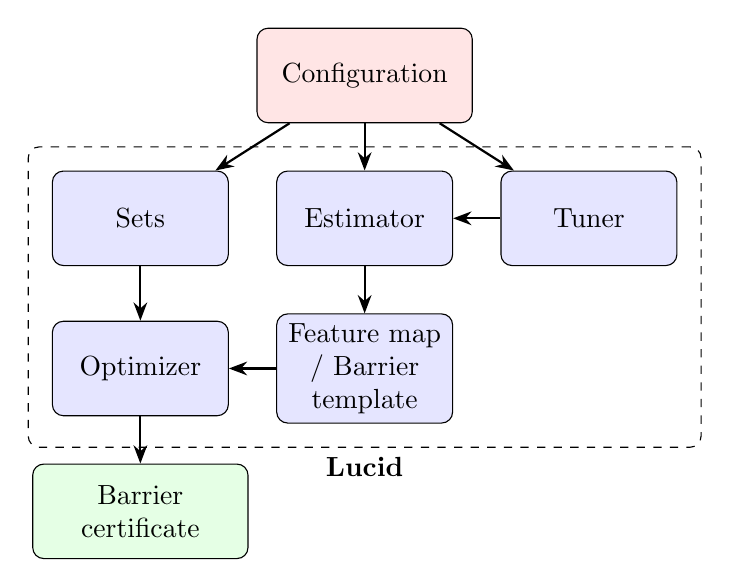
\begin{tikzpicture}[node distance=0.6cm and 0.6cm,
            input-block/.style={rectangle, draw, fill=red!10, text width=2.5cm, minimum height=1.2cm, align=center, rounded corners},
            output-block/.style={rectangle, draw, fill=green!10, text width=2.5cm, minimum height=1.2cm, align=center, rounded corners},
            block/.style={rectangle, draw, fill=blue!10, text width=2.0cm, minimum height=1.2cm, align=center, rounded corners},
            arrow/.style={thick,->,>=Stealth},
            tool/.style={rectangle, draw, fill=magenta!10, text width=3cm, minimum height=0.8cm, align=center, rounded corners},
            inv/.style={}
        ]

        % Input block
        \node[input-block] (input) {Configuration};

        % Lucid blocks
        \node[block, below=of input] (estimator) {Estimator};
        \node[block, right=of estimator] (tuner) {Tuner};
        \node[block, left=of estimator] (sets) {Sets};
        \node[block, below=of estimator] (feature) {Feature map / Barrier template};
        \node[block, left=of feature] (optimizer) {Optimizer};
        % \node[block, below=of optimizer] (verifier) {Verifier};
        \node[draw, dashed, inner sep=0.3cm, rounded corners,
        % fit=(estimator)(feature)(optimizer)(verifier), label=above:{\textbf{Lucid}}] {};
        fit=(estimator)(feature)(optimizer)(sets)(tuner), label=below:{\textbf{Lucid}}] {};

        % Output block
        % \node[output-block, left=of verifier] (output) {Barrier certificate};
        \node[output-block, below=of optimizer] (output) {Barrier certificate};

        % Smt solvers
        % \node[inv, below=2.5cm of verifier.north, anchor=north] (smtInv) {};
        % \node[tool, left=0.3cm of smtInv] (dreal) {dReal};
        % \node[tool, right=0.3cm of smtInv] (cvc5) {CVC5};
        % \node[draw, dashed, inner sep=0.3cm, rounded corners,
        % fit=(dreal)(cvc5), label=left:{\textbf{SMT Solver}}] {};

        % Arrows
        \draw[arrow] (input) -- (estimator);
        \draw[arrow] (input) -- (tuner);
        \draw[arrow] (input) -- (sets);
        \draw[arrow] (sets) -- (optimizer);
        \draw[arrow] (tuner) -- (estimator);
        \draw[arrow] (estimator) -- (feature);
        \draw[arrow] (feature) -- (optimizer);
        % \draw[arrow] (optimizer) -- (verifier);
        % \draw[arrow] (verifier) -- (output);
        \draw[arrow] (optimizer) -- (output);

        % \draw[arrow] (cvc5.north) -- (verifier.south);
        % \draw[arrow] (dreal.north) -- (verifier.south);

    \end{tikzpicture}
    \caption{General architecture of Lucid, highlighting its core components and their connections.}
    \label{fig:architecture}
\end{figure}


\subsubsection{Samples}

Due to its data-driven nature, all that \lucid needs to operate is a set of sampled trajectories from the system.
It can be obtained by defining a function that takes as input the current state and control input and returns the next state, adding an i.i.d. noise sampled from an appropriate distribution, or it may be collected from a simulator or a real-world system.
The sampled trajectories are then fed into \lucid, either programmatically, via a script that generates them on the fly, or through a file.
\pylucid natively supports \texttt{.csv}, \texttt{.mat}, \texttt{.npy} and \texttt{.npz} files. \todo{HDF5?}

\subsubsection{Sets}

\lucid understands \texttt{RectSet}s and \texttt{Multiset}s, i.e., a collection of sets.
These are used to indicate the bounds of the whole state space $\X$, the initial $\X_0$ set and the unsafe set $\X_u$ when defining the safety specification $\psi_{\text{safe}}$.
They also provide some utility methods for sampling and creating a lattice of the subspaces they define.

\subsubsection{Estimator}

The core of \lucid is its \texttt{KernelRidgeRegressor}, which uses a \texttt{GaussianKernel} to learn the underlying system dynamics from the samples.
Its predictions are then used to produce the next state of all the lattice points we need from $\X$, necessary to determine the constraints for the \gls{cbc}.

\subsubsection{Tuners}

Kernel methods do not require the expensive learning process of other machine learning methods, such as neural networks.
However, they still depend on a number of \hp, such as the kernel bandwidth $\sigma_f$ and the number of Fourier coefficients $M$.
Changes in their values can have a significant impact on the estimator's efficiency and accuracy.
The process of finding good values for these \hp is known as \emph{hyperparameter tuning}, and it is problem-dependent.
\lucid provides a set of utilities, which specialize the \texttt{Tuner} interface, to aid in this task.
A cheap starting point when working with a Gaussian Kernels as in~\eqref{eq:gaussian-kernel} is to use the \emph{median heuristic} \cite{garreau2018largesampleanalysismedian}, implemented in the \texttt{MedianHeuristicTuner}.
We choose $\sigma_l^2$ to be the median of the squared distances between all pairs of points in the training set, i.e.,
\begin{equation}
    \sigma_l^2 = \mathrm{median}_{1 \leq i < j \leq N}\left(\|\hat{x}_i-\hat{x}_j\|^2\right),
\end{equation}
where $\hat{x}_1,\ldots,\hat{x}_N$ are the $N$ training samples.
If $N(N-1)/2$ is even, the median is the average of the two middle values in the sorted list of distances.
The \texttt{GridSearchTuner}, on the other hand, implements the grid search method, exploring the space of possible \hp values to find the one that yields the best estimator $R^2$ score,
defined as $R^2 = 1 - \frac{\sum_{i=1}^n (y_i - \hat{y}_i)^2}{\sum_{i=1}^n (y_i - \bar{y})^2}$.
This approach is simple to implement and can be very effective for small problems, but it can become computationally expensive for larger ones.
Borrowing a technique from Gaussian processes, we can also optimize the \hp to maximize the \emph{log marginal likelihood}, defined as
\begin{equation}
    \begin{split}
        \log p(\hat{X^+}_N | \hat{X}_N) = & - \frac{1}{2}\hat{X^+}_N\T (K_{\hat{X}}^N + N\lambda I_N)^{-1} \hat{X^+}_N \\
        & -\frac{1}{2}\log |K_{\hat{X}}^N + N\lambda I_N| - \frac{N}{2}\log(2\pi).
    \end{split}
\end{equation}
To do so, the \texttt{LBFGSTuner} uses the L-BFGS or L-BFGS-B quasi-Newton optimization algorithms~\cite{book:nonlinear-programming},
implemented in the \texttt{LBFGS++} library~\footnote{https://github.com/yixuan/LBFGSpp}.

\subsubsection{Feature map}

We exploit the known expansion of the Gaussian kernel by building an explicit approximated feature map, composed of a linear sum of trigonometric functions with increasingly high frequencies.
The full expansion of the kernel would need a sum of infinite of terms with diminishing impact on the overall result, which we truncate arbitrarily short, a decision based on the tradeoff we are looking for between efficiency and accuracy.
After being defined with the same \hp that characterize the \texttt{KernelRidgeRegressor}, the function can be used to map any point from $\X$ to the \gls{rkhs} defined by the kernel.
\todo{link to the theory} There are currently three different ways the probability distribution can be divided in when associated to the frequency bands.
The whole interval can be divided equally, with a logarithmic scale or in smaller intervals with an arbitrary size.
Trying out different feature map implementations may yield different results.

\subsubsection{Barrier}

\todo{Barriers should probably be an explicit class in \lucid that hides the opitmisation implementation}
The finite-constraint relaxation of the SIP \eqref{eq:semiinf-prog} is what \lucid uses to synthesize the \gls{cbc} $\B$.
When verifying the safety of a system, \lucid will search for a \gls{cbc} $\B$ that satisfies the conditions in Definition~\ref{def:cbc}.
If it finds it, it will return the constants $\eta$, $\gamma$, and $c$, as well as the \gls{cbc} $\B$ itself, which becomes a certificate of safety for the system $\M$.
More precisely, we follow the steps outlined in~\ref{fig:steps}.
While the theory gives us precise indication on how to construct the \gls{lp} which would yield a correct-by-design solution,
in practice the constraints may prove to be too conservative.
To mitigate this, the user can either increase the number of lattice points $Q$, worsening the computational efficiency,
or adjust the coefficient $C_{\hat{N}}$, improving performance at the cost of loosening the guarantees.
The resulting barrier can then be checked with the verifier, provided we have access to the system's model, to ensure its correctness.
\lucid can be configured to work with any of the following linear optimisers: \gurobi, \alglib or \highs.

\section{Configuration}

The recommended way to use \lucid is through its Python wrapper \pylucid.
After being installed, it can be invoked from the command line with \lstinline|pylucid|.
For define the scenario to run, we suggest using a \yaml or equivalent \json file~
\footnote{The Json schema for \yaml and \json files can be found at \url{https://tendto.github.io/lucid//configuration_schema.json}} like

\lstinputlisting[language=yaml,caption={\texttt{example.yaml} configuration file.}]{code/linear.yaml}

The same configuration values can also be given to the executable directly as command line arguments.
For a list of all available options, run \lstinline|pylucid --help|.
If more flexibility is needed, a python script can be provided instead,
with the only requirement being that it must contains a function named \lstinline|scenario_config| returning \texttt{Configuration} object.
Any configuration can be loaded with the command \lstinline|pylucid <config file>|.
Lastly \pylucid also provides a \gls{gui} to guide the user in the creation of the scenario configuration and presenting the results in an intuitive way.
To start the \gls{gui}, make sure to have installed the necessary dependencies with \lstinline|pip install pylucid[gui]| \todo{Installation guide?} and run the command \lstinline|pylucid-gui|.
This will open a browser tab containing the interface, while a local server will listen for requests coming from the \gls{gui}, returning the results.
\todo{picture of the GUI}

\section{Functionality}

Having parsed and validated the scenario configuration, \lucid will begin the main pipeline to produce the expected result.
If a set of sample transitions has not been provided by the user, \lucid will try to produce it itself by randomly sampling $\X$ to which apply the system dynamics function.
The samples will be used to fit and optionally tune the estimator so that, given an input state, it will accurately predict the value of the feature map applied to the next state.
\lucid will then store a lattice of points from each of the set provided to which apply the feature map.
These values will finally be used to define the constraint of the \gls{lp} that the chosen optimizer will solve.
The solution, if found, will determine the barrier certificate coefficients, as well as the satisfaction probability.
\lucid provides the option to employ the \dreal SMT solver to verify the barrier formally if the system dynamics are known.

\begin{figure}[ht]
    \centering
    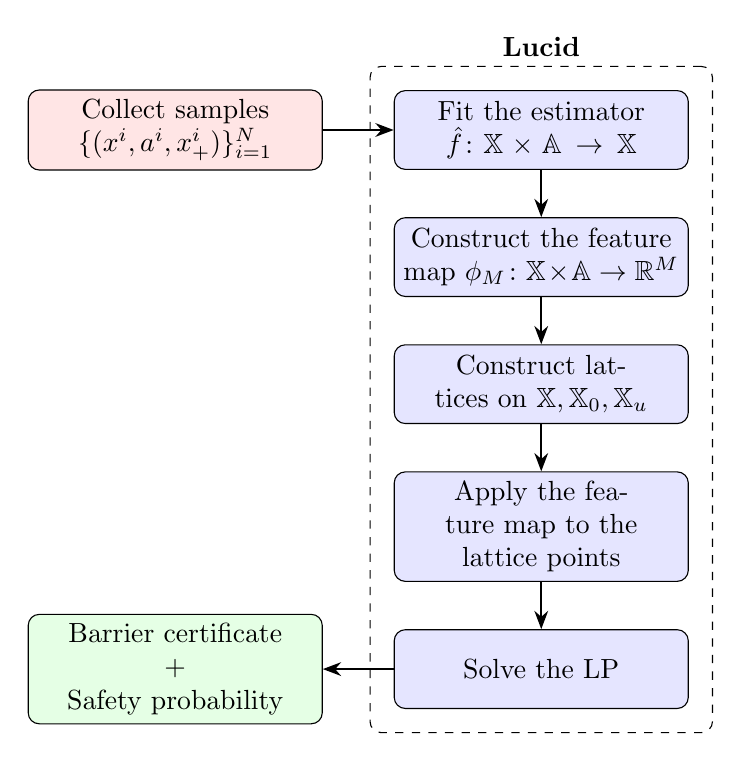
\begin{tikzpicture}[node distance=0.6cm and 0.9cm,
            input-block/.style={rectangle, draw, fill=red!10, text width=3.5cm, minimum height=1.0cm, align=center, rounded corners},
            output-block/.style={rectangle, draw, fill=green!10, text width=3.5cm, minimum height=1.0cm, align=center, rounded corners},
            block/.style={rectangle, draw, fill=blue!10, text width=3.5cm, minimum height=1.0cm, align=center, rounded corners},
            arrow/.style={thick,->,>=Stealth},
            tool/.style={rectangle, draw, fill=green!20, text width=2cm, minimum height=0.8cm, align=center, rounded corners},
            inv/.style={}
        ]

        % Input block
        \node[input-block] (input) {Collect samples $\{(x^i,a^i, x_+^i)\}_{i=1}^N$};

        % Lucid blocks
        \node[block, right=of input] (estimator) {Fit the estimator $\hat{f}\colon \X\times\A \to \X$};
        \node[block, below=of estimator] (feature) {Construct the feature map $\phi_M\colon \X\times\A \to \mathbb{R}^M$};
        \node[block, below=of feature] (lattice) {Construct lattices on $\X, \X_0, \X_u$};
        \node[block, below=of lattice] (apply-lattice) {Apply the feature map to the lattice points};
        \node[block, below=of apply-lattice] (optimizer) {Solve the LP};
        \node[draw, dashed, inner sep=0.3cm, rounded corners,
        fit=(estimator)(feature)(lattice)(apply-lattice)(optimizer), label=above:{\textbf{\lucid}}] {};

        % Output block
        \node[output-block, left=of optimizer] (output) {Barrier certificate\\+\\Safety probability};

        % Arrows
        \draw[arrow] (input) -- (estimator);
        \draw[arrow] (estimator) -- (feature);
        \draw[arrow] (feature) -- (lattice);
        \draw[arrow] (lattice) -- (apply-lattice);
        \draw[arrow] (apply-lattice) -- (optimizer);
        \draw[arrow] (optimizer) -- (output);

    \end{tikzpicture}
    \caption{Sequence of steps \lucid goes through to generate a barrier certificate.}
    \label{fig:steps}
\end{figure}


\section{Experimental Evaluation}
Overview of the experimental results in Table~\ref{tbl:benchmarks_results}.
\begin{table}[tb]
    \centering
    \begin{tabular}{ccccc}
        \toprule
        \textbf{Benchmark} & \textbf{Dim} & \textbf{\#LatP} & \textbf{Runtime} & \textbf{Safety Prob.} \\
                           &              &                 & [mm:ss]          & [\%]                  \\ % Units
        \midrule
        Linear             & 1            &                 & X:XX             & XX                    \\
        Barr3              & 2            & $30^2$          & X:XX             & XX                    \\
                           &              & $40^2$          & X:XX             & XX                    \\
        Overtaking         & 3            &                 & X:XX             & XX                    \\
        name2              & 7            &                 & X:XX             & XX                    \\
        \bottomrule
    \end{tabular}
    \caption{Computational benchmarks: ...}
    \label{tbl:benchmarks_results}
\end{table}

\begin{figure}
    \centering
    \includegraphics[width=\linewidth]{placeholder.jpeg}
    \caption{Barrier}
    \label{fig:barr3_barrier}
\end{figure}

\section{Conclusion}


%%%%%%%%%%%%%%%%%%%%%%%%%%%%%%%%%%%%%%%%%%%%
%%%%%%%%%%%%%%%%%%%%%%%%%%%%%%%%%%%%%%%%%%%%
%%%%%%%%%%%%%%%%%%%%%%%%%%%%%%%%%%%%%%%%%%%%
\bibliography{aaai25}

\end{document}
